% the following line is added to eliminate warnings about fonts on Mac
\PassOptionsToPackage{quiet}{fontspec} 

% use ctexarticle and include own package hw-cn.sty
\documentclass[]{ctexart}
\usepackage{hw-cn}

\usepackage{inputenc}
\usepackage{amsfonts,amsmath,amscd,amssymb,amsthm}
\usepackage{latexsym,bm}
\usepackage{cite}
\usepackage{mathtools,mathdots,graphicx,array}
\usepackage{fancyhdr}
\usepackage{lastpage}
\usepackage{color}
\usepackage{enumitem}
\usepackage{diagbox}
\usepackage{xcolor,tcolorbox,tikz,tkz-tab,mdframed,tikz-cd}
\usepackage{framed}
\usepackage{verbatim}
\usepackage{extarrows}
\usepackage{fontspec}
\usepackage{subfigure}
\usepackage{float} % use H command to fix position of figures
\usepackage{graphicx}
\usepackage{listings}
\usepackage{hyperref}
\usepackage{makecell}
\usepackage{bbding}


\newcommand\course{智能感知认知实践}
\newcommand\taskinfo{任务}
\newcommand\name{孙一林}
\newcommand\stuID{520030910361}

\pagestyle{fancyplain}
\headheight 25pt
\lhead{\name \\ \stuID}
\chead{\textbf{\Large 图片摘要生成\taskinfo}}
\rhead{\course \\ \today}

\begin{document}

\section{提交说明和简介}

\subsection{提交简要说明}
本次任务使用实验室服务器进行实验,在超算提供代码的基础上,更改了\texttt{model.py}以在Captioner中实现Scheduled Sampling,
为了配置新的超参数,对\texttt{main.py}进行了相应的修改,除此之外保留了原有的代码框架,在训练过程中根据参数配置修改了\texttt{config}文件,
并在其中添加了\texttt{use\_ss}选项,即使用scheduled\_sampling的选项,设置为\texttt{true}时即使用,从而与原有的模型训练逻辑进行实验对比。
实验结果保留在\texttt{experiments}文件夹下。

\subsection{任务简介}
图片摘要生成是综合计算机视觉和自然语言处理的一个跨模态任务,它的目的是使计算机尝试理解图像的内容,以生成与对图像的概括总结性质的文本描述。
由于这是一个跨模态任务,我们可以利用神经网络对输入数据集生成的摘要文本来观察模型对图像的理解程度,在此基础上也可以帮助我们更好地理解计算机视觉任务中一些潜在的问题和发展空间。
除此之外,图片摘要生成还有着比较重要的应用价值,图片摘要可以被认为是一种对图像信息在语义层面上的压缩,得到的并非传统计算机视觉中对输入数据处理得到的feature map,
而是人能够理解的自然语言,从这个角度而言,对于图片摘要生成的结果不但可以用客观指标来进行评测,还可以用主观理解进行评估。

为了能够解决图片摘要生成任务,必然要使用跨模态神经网络模型,以汇总和融合图像、文本数据,并尝试解读数据之间的相关性。
对于处于不同模态的数据,本次实验采取在单模态数据中功能得到普遍验证的Encoder-Decoder框架来进行。

本次任务使用Flicker8k数据集,该数据集提供跨模态数据,除了图像之外,每张图片还提供了五条人工标注的图片摘要。
本次实验使用的评价指标主要有Bleu-1、Bleu-2、Bleu-3、Bleu-4、Rouge、METEOR、CIDEr、SPICE、SPIDEr,实验部分会详述。

\section{任务理解}
本部分将在描述编码器-解码器模型的整体框架的同时,解释跨模态模型对于不同模态数据处理的方式,并描述scheduled sampling的原理。

整体而言,由于我们的任务是图片摘要,上游输入是图像类数据,下游输出是文本类数据,那么对于上游输入而言,
首先使用Encoder以提取图像的隐层信息,尝试得到图片语义信息的较好表示;之后再将中间结果输入Decoder以生成下游的文本信息,并进行观察和评估。
考虑到处理图片信息,Encoder可以使用卷积神经网络等图像特征提取模型;同样地,考虑到处理文本信息,Decoder可以使用循环神经网络来捕获和表达语义信息。

\subsection{编码器Encoder}
Captioner的Encoder模块主要负责将输入的图像编码成特征向量,以供后续的图片摘要生成过程使用。
Encoder模块可以使用一些目前已经在广泛的任务上被证明具有良好性能的神经网络,本次实验推荐使用ResNet101.
ResNet通过具有多个层次的卷积层和跳跃连接以有效地提取图像特征,并将输入图像转换为特征向量。
ResNet相比于传统神经网络而言,引入了残差学习的方式,提高了深度神经网络的可训练性,并一定程度上解决了深度网络的退化问题。
在本次实验的环境下,ResNet101能够取得不错的效果。

\subsection{基于注意力的解码器DecoderWithAttention}
Captioner的DecoderWithAttention模块用于将提取好的语义信息解码为文本摘要。
它可以使用基于循环神经网络的解码器架构,例如长短期记忆网络,通过被称为遗忘门、输入门和输出门的三个门来控制信息上下文在神经元之间的流动。
除此之外,他还结合了注意力机制来动态地选择图像特征的相关部分,通过结合先前已经生成的文本摘要信息,并在每个时间步上引入注意力机制,
在每一个时间步下,Decoder都可以结合当前时间和先前时间步的状态信息,动态地计算出注意力上的权重,
在此之后,可以将得到的图像特征进行注意力加权,再与先前的隐藏状态结合,最终产生一个输出并传递给下个时间步。

\subsection{搜索策略}
仅仅使用Encoder和Decoder提取和解码信息是不够的,Captioner还需要基于一定的搜索策略来生成最终的文本摘要。
在本次实验的配置下,Captioner可以选择Greedy和Beam两种不同的搜索策略,以得到摘要文本。
Greedy搜索策略简单高效、直观易懂,在每个时间步上,Captioner都会有多个不同的单词可以选取,这时候他就贪婪地选择具有最高概率的单词作为下一个时间步的输出。
通过这种简单的贪婪策略,Captioner已经能够方便地获得不错的结果,且这种方式比较易于实现;
相应地,这种策略也更容易会得到局部最优的答案,在很多情况下都不能得到全局最优解。

在此基础上,更复杂的Beam搜索策略通过设定一个合理大小的搜索空间,保留多个可能的文本序列,根据概率对它们进行排序和筛选。
通过控制搜索空间的大小,Beam搜索策略可以兼顾搜索的开销和全局的准确度,从而给出全局上来说语义信息更加准确的文本摘要。

\subsection{Scheduled Sampling}
Scheduled Sampling是一种用于训练Captioner中Decoder的技术,通过概率性地选取真实目标和自己生成的单词,来减轻训练期间Teacher Forcing和推断期间替代采样之间的差异。
Teacher Forcing原论文中提到的训练技术,在每个时间步上将真实的目标单词作为输入传入解码器。在有监督的情况下,每一时刻的输入前一个单词都是一个ground truth,
而未知的前一个单词会被模型自己生成的单词替换,所以训练和推断之间由此产生了差异,也就会进一步产生误差,当模型在推断阶段使用自己生成的单词作为输入时,这些误差便会沿着产生的单词序列累积。
也就是说,如果在推理阶段的某一时刻单词计算错误,这个错误就会由当前的生成序列传递下去。

为了解决这个问题,Scheduled Sampling的策略是逐渐增加模型使用自己生成的单词的概率。
在训练期间,模型并不会完全使用真实的目标单词,而是以一定的概率使用,而同时以一定的概率使用自己生成的单词作为输入。
模型可以控制并逐渐增加自我生成单词的使用概率,以便在训练阶段就对推理阶段可能出现的单词做出一定的准备。

\section{实验}

\subsection{数据集}
本次实验使用Flicker8k数据集。Flicker8k数据集是Flicker系列下的一个数据集,其中包含了8000张图片及其配套的摘要,在\texttt{caption.txt}文件中,
每张图片提供了5个标注好的摘要,以综合地概括图片的语义信息。
数据集配置已经预划分为训练集、验证集和测试集,并通过\texttt{.txt}文件标注了对应的文件名。

\subsection{评估指标}
对于跨模态任务而言,由于数据来自不同模态,单一的评估指标往往不能全面地评估模型性能的好坏,所以需要综合多个不同的评估指标来考察。
通过调研,本次实验我们用到的相关评估指标和他们的作用如下:
\begin{itemize}
    \item Bleu-n:基于n-gram匹配的评价指标,用于衡量生成的摘要与参考摘要之间的相似性。其中n则是n-gram中的长度,本次实验中n取[1-4]
    \item Rouge:一种面向召回率的评价指标,与Bleu类似,也能衡量生成的摘要与参考摘要之间的相似性。
    \item METEOR:结合了精确度、召回率和一致性的评价指标。通过计算特定的序列匹配,同义词、词根、词缀、释义之间的匹配关系,改善了Bleu的效果,使其跟人工判别有更强的相关性。
    \item CIDEr:结合了Bleu和向量空间模型的评价指标。它将每个句子看成一个文档,计算其n-gram的TF-IDF向量,再用余弦相似度来衡量候选句子和参考句子的语义一致性。其优点是能够捕捉到不同长度的n-gram之间的匹配,而且可以通过TF-IDF权重来区分不同n-gram的重要性。
    \item SPICE:使用基于图的语义表达来编码摘要中的对象、特征和关系,在评估时名词的相似度会得到更多的重视。
    \item SPIDEr:主要考察生成的摘要与参考摘要之间的语义一致性的评估指标。
\end{itemize}

\subsection{实验结果}
\begin{table}[ht]
    \centering
    \begin{tabular}{|c|c|c|c|c|c|c|c|c|c|c|c|c|}
      \hline
        \diagbox{Model}{Metrics}
        &Bleu-1&Bleu-2&Bleu-3&Bleu-4&Rouge&METEOR&CIDEr&SPICE&SPIDEr\\
        \hline
        Res+Att&0.583&0.396&0.262&0.172&0.405&\textbf{0.195}&0.473&\textbf{0.143}&0.308\\
        \hline
        Res+Att+SS&\textbf{0.603}&\textbf{0.410}&\textbf{0.273}&\textbf{0.176}&\textbf{0.407}&0.192&\textbf{0.485}&0.139&\textbf{0.312}\\
        \hline
    \end{tabular}
    \caption{是否启用scheduled sampling的实验结果对比}
    \label{result}
\end{table}
上述表格中的SS即指Scheduled Sampling的开启。
从结果中可以看到,在使用了Scheduled Sampling的情况下,各项指标均有着一定的提升,只有METEOR和SPICE指标和
不使用Scheduled Sampling的情况下略有微小的下降,可以看出,使用Scheduled Sampling来调整Decoder读单词的选取策略确实能够带来性能上的提升。
\subsection{图片摘要分析}
本节选取部分图片生成结果,给出其ground truth中较有代表性的图片摘要,并分析不同方法下的生成结果。

本节中Ground Truth标注在图片下方。
\begin{figure}[ht]
    \centering
    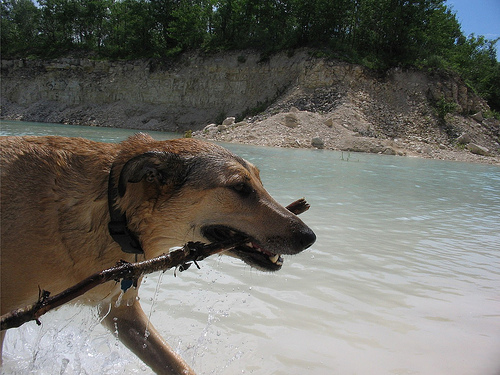
\includegraphics[width=0.8\textwidth]{asset/352382023_7605223d1c.jpg}
    \caption{A dog carrying a stick while walking in water.}
    \label{demo1}
\end{figure}

不同方法下的摘要生成结果为:
\begin{itemize}
    \item Baseline: dog is jumping into the water .
    \item Scheduled Sampling added: brown dog is jumping into the water .
\end{itemize}
可以看到,两种方法都不能完全还原图片中的语义信息,但是在Scheduled Sampling启用的情况下,Captioner能够从原图中捕获更多的信息,即能够提取物体的颜色(棕色的狗)。
通过观察更过的摘要生成结果我发现,启用了Scheduled Sampling的情况下Captioner对于颜色的提取并不总是准确的,但是确实能够提供更丰富的文本摘要信息。

\newpage
\begin{figure}[ht]
    \centering
    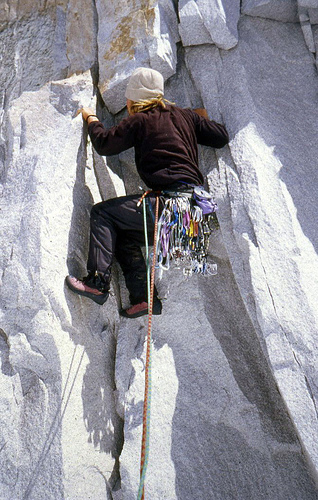
\includegraphics[width=0.4\textwidth]{asset/486917990_72bd4069af.jpg}
    \caption{A person wearing a white hat climbs a rock.}
    \label{demo2}
\end{figure}
不同方法下的摘要生成结果为:
\begin{itemize}
    \item Baseline: man is climbing up a rock face .
    \item Scheduled Sampling added: man in a white shirt and a white shirt is climbing a rock face .
\end{itemize}
此即Scheduled Sampling启用的Captioner对图片中信息错误提取的一个例子。
原图中给出的Ground Truth指出图片中的人物戴着白色的帽子,不使用Scheduled Sampling的情况下,
Captioner会直接忽略这一信息(可能这个相对而言信息也是不关键的),使用了Scheduled Sampling时,Captioner则会错误地认为人穿了一件白色的衬衫,
这样一个信息的提取可能是因为考虑到了环境的因素,即整个山的背景呈白色;也有可能是因为人携带的装备主要呈白色。
但是Captioner确实没有识别出人物真实的衬衫颜色(棕色)。

\end{document}